\documentclass[a4paper,12pt]{article}

\usepackage[utf8]{inputenc}
\usepackage[T1]{fontenc}
\usepackage[margin=2.5cm]{geometry}
\usepackage{graphicx}
\graphicspath{{images/}}

\usepackage{listings}
\usepackage{xcolor}
\usepackage{amsmath}
\usepackage{enumitem}
\usepackage{url}

\lstset{
	language=Python,
	basicstyle=\ttfamily\small,
	keywordstyle=\color{blue},
	commentstyle=\color{gray},
	stringstyle=\color{red},
	showstringspaces=false,
	breaklines=true,
	frame=single
}

\setlength{\emergencystretch}{3em}

\begin{document}
	
	\section*{Part 1 -- Python and Object-Oriented Programming}
	
	\subsection*{Q1. What are the entities in our academic model?}
	
	\textbf{Answer:}
	
	The main entities in our academic model are Semester, Teaching Unit (Unit / UE), Module, and Student.
	
	A module contains a code or name, a title, a coefficient, credits, weekly lecture/TD/TP hours, teaching mode, evaluation percentages, and grades. A unit contains modules, and a semester contains units. A student receives grades and accumulates credits.
	
	\subsection*{Q2. Create and test the Module class.}
	
	\textbf{Answer:}
	
	The \texttt{Module} class stores module information, calculates the total semester workload as
	\[
	15 \times (\text{lecture}+\text{TD}+\text{TP}),
	\]
	stores grades, prints a summary, and provides methods for calculating the average and credits.
	
	\textbf{Screenshot :}
	
	 \begin{center}
		  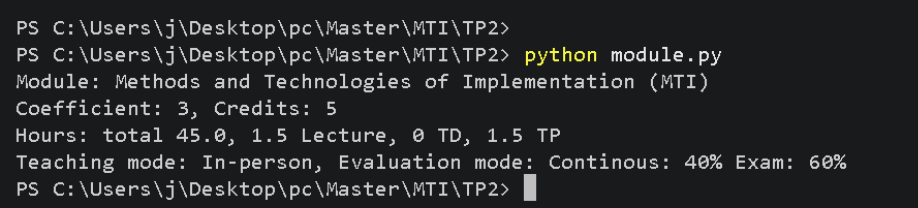
\includegraphics[width=0.8\textwidth]{photo1.png}
	 \end{center}
	
	\subsection*{Q3. Implement \texttt{calculate\_average()} and \texttt{calculate\_credits()}.}
	
	\textbf{Answer:}
	
	The continuous-assessment percentage is split equally between TP and TD when both exist. If only one exists, it receives the full continuous-assessment percentage. The exam receives the examination percentage.
	
	Credits are awarded if the module average is at least \(10/20\). Otherwise, the module earns zero credits.
	
	\textbf{Screenshot :}
	
	 \begin{center}
		   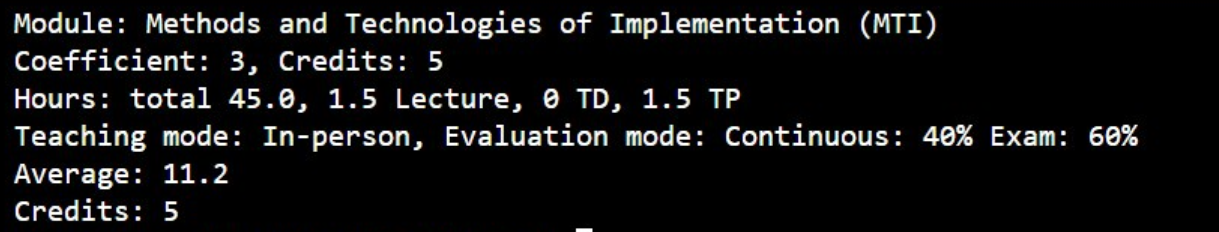
\includegraphics[width=0.8\textwidth]{photo2.png}
	 \end{center}
	
	\subsection*{Q4. Implement the Unit class.}
	
	\textbf{Answer:}
	
	The \texttt{Unit} class inherits from \texttt{AcademicElement} and stores a collection of \texttt{Module} objects. The method \texttt{add\_module(module)} adds a module to that collection.
	
	\textbf{Code link:}
	
	% Replace with your actual URL, if applicable.
	% \url{https://example.com}
	
	\subsection*{Q5. Identify similarities between Unit and Module.}
	
	\textbf{Answer:}
	
	Both are academic elements and share common attributes, such as name, title, coefficient, credits, and workload attributes. They must also implement average and credit calculations.
	
	A \texttt{Module} stores grades and evaluation rules, whereas a \texttt{Unit} aggregates multiple modules.
	
	\subsection*{Q6. Explain the inheritance relationship between Unit and Module.}
	
	\textbf{Answer:}
	
	A \texttt{Unit} should not inherit from \texttt{Module}, and a \texttt{Module} should not inherit from \texttt{Unit}, because a unit is not a module and a module is not a unit.
	
	Both classes inherit from the common abstract parent \texttt{AcademicElement}. The relationship between \texttt{Unit} and \texttt{Module} is containment or aggregation.
	
	\subsection*{Q7. Why use abstract \texttt{AcademicElement} and test the code?}
	
	\textbf{Answer:}
	
	The \texttt{AcademicElement} class centralizes common attributes and declares \texttt{calculate\_average()} and \texttt{calculate\_credits()} as abstract methods.
	
	A subclass must implement these methods. In Python, the class must inherit from \texttt{ABC} and import \texttt{abstractmethod} from the \texttt{abc} module to enforce the abstract-method requirements.
	
	\textbf{Screenshot (optional):}
	
	% \begin{center}
		%   \includegraphics[width=0.8\textwidth]{photooooo.png}
		% \end{center}
	
	\subsection*{Q8. Can Semester be a subclass under the abstraction principle?}
	
	\textbf{Answer:}
	
	Yes. A \texttt{Semester} is also an \texttt{AcademicElement}, so it can inherit from \texttt{AcademicElement} and implement its own average and credit calculation methods. A semester contains units.
	
	\subsection*{Q9. Check encapsulation in Module and modify it if necessary.}
	
	\textbf{Answer:}
	
	The original \texttt{\_grades} dictionary is protected by convention, rather than strictly private.
	
	The \texttt{set\_grade()} method controls grade updates, and the average calculation method reads the grades internally.
	
	The corrected implementation validates grades between 0 and 20 and raises a clear error if required grades have not been supplied, instead of failing with a \texttt{None} arithmetic error.
	
	\subsection*{Q10. Override \texttt{calculate\_average()} and \texttt{calculate\_credits()} for Unit.}
	
	\textbf{Answer:}
	
	The unit average is the coefficient-weighted mean of its module averages:
	\[
	\text{Unit Average}
	=
	\frac{
		\sum_{i=1}^{n}
		\left(\text{Module Average}_i \times \text{Module Coefficient}_i\right)
	}{
		\sum_{i=1}^{n}\text{Module Coefficient}_i
	}.
	\]
	
	If the unit average is at least 10, all credits of its modules are counted. Otherwise, only the credits earned by modules individually are counted. An empty unit returns an average of zero.
	
	\subsection*{Q11. Define Semester and implement its methods.}
	
	\textbf{Answer:}
	
	The \texttt{Semester} class contains units. Its average is calculated as the coefficient-weighted mean of the unit averages. Its credits are the sum of the credits earned by its units.
	
	This implementation assumes that each unit's coefficient is the sum of its module coefficients.
	
	\textbf{Screenshot and code link (optional):}
	
	% \begin{center}
		%   \includegraphics[width=0.8\textwidth]{photoo.png}
		% \end{center}
	% Replace the URL below with your actual link:
	% \url{https://example.com}
	
	\subsection*{Q12. Implement the whole GSI Canvas logic.}
	
	\textbf{Answer:}
	
	Implement the main application logic in \texttt{main.py}. The program should integrate the academic elements, manage students, and test the interaction between the different classes.
	
	The implementation should allow students to be added and should verify that the academic model works correctly.
	
	\textbf{Main program placeholder:}
	
	\begin{lstlisting}
		# main.py
		# Implement the complete GSI Canvas logic here.
		# Add students and test the academic model.
	\end{lstlisting}
	
\end{document}
